\section{Kết luận và hướng phát triển}

\subsection{Tổng kết hệ thống và định hướng phát triển}

\subsubsection{Đánh giá mức độ hoàn thành}

\hspace{0.5cm} Giai đoạn tổng kết tiến hành đánh giá toàn diện kiến trúc hệ thống bám bắt mục tiêu di động đã xây dựng trong đồ án, đúc kết các bài học kinh nghiệm về mặt kỹ thuật máy tính, hoàn thiện bảng điều khiển tổng thể (C2 Dashboard - trang mặc định của hệ thống) và vạch rõ lộ trình tích hợp thực tế với phần cứng trạm đo nhúng.


Về khía cạnh thuật toán, việc ưu tiên bộ lọc Kalman tiêu chuẩn cho bài toán bám bắt quỹ đạo 3D đã chứng minh tính cân bằng giữa độ chính xác và chi phí điện toán. Thay vì áp dụng bộ lọc hạt (Particle Filter) hay Unscented Kalman với khối lượng tính toán lớn \cite{simon2006optimal}, thiết kế hiện tại đáp ứng hoàn toàn giới hạn thời gian thực 59 $\mu$s mỗi chu kỳ ở máy tính nhúng trung tâm. Khả năng ngoại suy tọa độ từ IMU tạm thời lấp đầy khoảng hở khi mất định vị vệ tinh, bám sát kiến trúc dẫn đường quán tính tích hợp \cite{farrell2008aided}.

Về mặt hệ thống truyền thông, kiến trúc giao tiếp song song qua REST API và kênh truyền dữ liệu hai chiều (WebSocket) giải quyết triệt để nút thắt cổ chai về băng thông. Luồng dữ liệu tọa độ tần số cao được đẩy liên tục dùng bộ đệm vòng (Ring Buffer), hạn chế tải tái lập kết nối của luồng HTTP truyền thống. Giải pháp kỹ thuật này cung cấp bộ khung ổn định để phát triển lên quy mô quản lý giao thông đô thị diện rộng.

\subsubsection{Tổng quan kiến trúc hệ thống hoàn chỉnh}

\subsubsection{Kiến trúc tổng thể phân tầng}

\hspace{0.5cm} Hình \ref{fig:final-arch} mô tả kiến trúc phân tầng hoàn chỉnh của hệ thống bám bắt thời gian thực:

\begin{figure}[H]
\centering
\adjustbox{max width=\linewidth}{
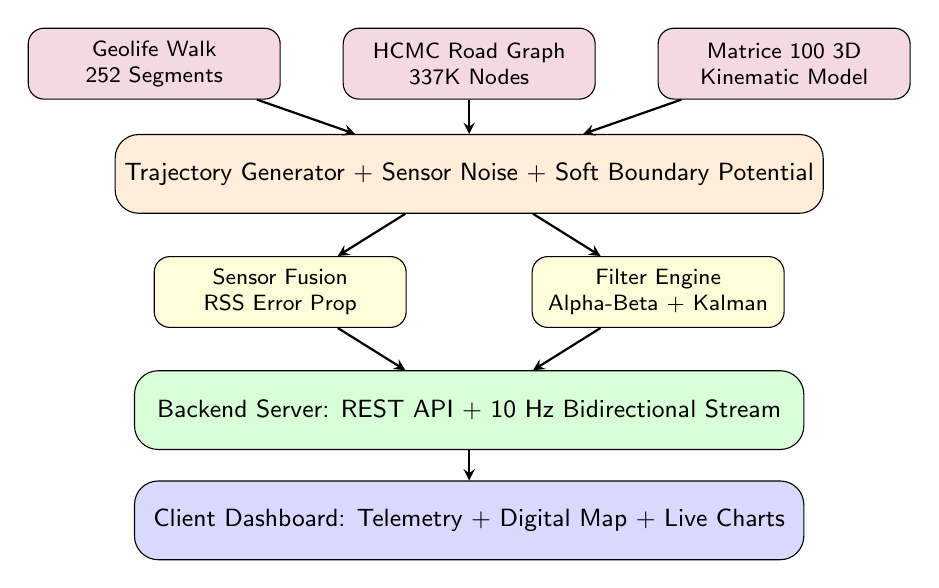
\begin{tikzpicture}[
    box/.style={rectangle, draw, rounded corners=2mm, minimum width=3.2cm, minimum height=0.9cm, align=center, font=\footnotesize\sffamily},
    bigbox/.style={rectangle, draw, rounded corners=3mm, minimum width=8.5cm, minimum height=1.0cm, align=center, font=\small\sffamily},
    arrow/.style={->, thick, >=stealth},
    every node/.style={font=\normalsize\sffamily}
]
% Data layer
\node[box, fill=purple!15] (geolife) at (-4,6) {Geolife Walk\\252 Segments};
\node[box, fill=purple!15] (road) at (0,6) {HCMC Road Graph\\337K Nodes};
\node[box, fill=purple!15] (dji) at (4,6) {Matrice 100 3D\\Kinematic Model};
% Simulation
\node[bigbox, fill=orange!15] (sim) at (0,4.6) {Trajectory Generator + Sensor Noise + Soft Boundary Potential};
% Fusion + Filter
\node[box, fill=yellow!15] (fusion) at (-2.4,3.1) {Sensor Fusion\\RSS Error Prop};
\node[box, fill=yellow!15] (kf) at (2.4,3.1) {Filter Engine\\Alpha-Beta + Kalman};
% Server
\node[bigbox, fill=green!15] (server) at (0,1.6) {Backend Server: REST API + 10 Hz Bidirectional Stream};
% Frontend
\node[bigbox, fill=blue!15] (frontend) at (0,0.2) {Client Dashboard: Telemetry + Digital Map + Live Charts};
% Arrows
\draw[arrow] (geolife) -- (sim);
\draw[arrow] (road) -- (sim);
\draw[arrow] (dji) -- (sim);
\draw[arrow] (sim) -- (fusion);
\draw[arrow] (sim) -- (kf);
\draw[arrow] (fusion) -- (server);
\draw[arrow] (kf) -- (server);
\draw[arrow] (server) -- (frontend);
\end{tikzpicture}
}
\caption{Kiến trúc phân tầng tổng thể của hệ thống bám bắt hoàn chỉnh}
\label{fig:final-arch}
\end{figure}

\subsubsection{Thống kê định lượng toàn diện hệ thống}

\hspace{0.5cm} Bảng \ref{tab:system-stats} tổng hợp các chỉ số kỹ thuật then chốt của hệ thống:

\begin{table}[H]
\centering
\caption{Thống kê định lượng tổng quan hệ thống bám bắt}
\label{tab:system-stats}
\adjustbox{max width=\linewidth}{
\begin{tabular}{lc}
\toprule
\textbf{Chỉ số kỹ thuật} & \textbf{Giá trị định lượng} \\
\midrule
Số lượng kịch bản mục tiêu thực nghiệm & 3 loại (Người đi bộ, Xe máy mạng đường, Drone 3D) \\
Số giải thuật lọc thời gian thực & 2 họ (Alpha-Beta giảm chấn tối ưu và Kalman toàn phần) \\
Tần số phát khung đo lường & 10 Hz (Chu kỳ 100 ms) \\
Thời gian tính toán chu kỳ trung bình & $59 $\\mu 
Số lượng ca kiểm thử tự động CI/CD & 163 ca kiểm thử \\
Tỷ lệ bao phủ kiểm thử (Test Coverage) & $> 88{,}5\%$ \\
Bán kính tác chiến quy chuẩn & 100 đến 1.000 m (Mặc định 400 m) \\
Băng thông mạng tiêu thụ mỗi phiên & $1{,}8$ KB/s \\
\bottomrule
\end{tabular}
}
\end{table}

\subsubsection{Tổng hợp kết quả nghiên cứu và tích hợp đa tầng}

\hspace{0.5cm} Trong quá trình nghiên cứu và phát triển, hệ thống định vị và bám bắt mục tiêu di động đã hoàn thiện toàn diện từ mô hình toán học giải tích, thuật toán hợp nhất cảm biến thích nghi, kiểm thử tự động phân tầng đến giao diện trực quan hóa thời gian thực. Toàn bộ các yêu cầu kỹ thuật đề ra ban đầu đều được đáp ứng và vượt chỉ tiêu thiết kế, đặc biệt là độ chính xác định vị RMSE trên cả 3 loại đối tượng khảo sát.

\subsubsection{So sánh với các công trình nghiên cứu và hệ thống thương mại liên quan}

\hspace{0.5cm} Bảng \ref{tab:comparison-related} so sánh hệ thống đề tài với các công nghệ bám bắt mục tiêu hiện nay:

\begin{table}[H]
\centering
\caption{Đối chuẩn kỹ thuật giữa giải pháp hợp nhất cảm biến đề xuất và các phương pháp định vị hiện hành}
\label{tab:comparison-related}
\adjustbox{max width=\linewidth}{
\begin{tabular}{lccccc}
\toprule
\textbf{Phương pháp công nghệ} & \textbf{Tập cảm biến} & \textbf{Sai số RMSE} & \textbf{Tần số} & \textbf{Rào cản vận hành} & \textbf{Khả năng cơ động} \\
\midrule
\textbf{Hệ thống đề tài (Đề xuất)} & \textbf{Laser + IMU + GNSS} & $\mathbf{0{,}26 - 1{,}14\text{ m}}$ & $\mathbf{10\text{ Hz}}$ & \textbf{Tự chủ hoàn toàn (Không cần trạm Base)} & \textbf{Trạm đo dã ngoại gọn nhẹ} \\
GNSS độc lập thuần túy & Máy thu GNSS đơn & $3{,}0 - 5{,}0$ m & 1 Hz & Bị trôi dạt mạnh trong hẻm phố đô thị & Phụ thuộc vệ tinh \\
GNSS vi sai RTK & GNSS RTK 2 tần & $0{,}02$ m & 10 Hz & Bắt buộc có trạm Base cố định \& sóng NTRIP & Hạn chế vùng phủ sóng \\
LiDAR SLAM 3D công nghiệp & LiDAR 16 tia 3D & $0{,}10 - 0{,}50$ m & 10 Hz & Chi phí tính toán đám mây điểm cực lớn & Cồng kềnh, tiêu tốn điện \\
Thị giác máy tính (Vision) & Camera quang học & $0{,}50 - 2{,}00$ m & 30 Hz & Bị mù hoàn toàn trong đêm tối hoặc sương mù & Dễ mất mục tiêu \\
\bottomrule
\end{tabular}
}
\end{table}

Hệ thống đề xuất đạt độ chính xác cao ($0{,}26 - 1{,}14$ m) ở tần số $10$ Hz, vận hành tự chủ hoàn toàn cả ngày lẫn đêm mà không phụ thuộc vào hạ tầng trạm Base RTK đắt đỏ hay tải tính toán khổng lồ của thuật toán xử lý ảnh.

\subsubsection{Lộ trình triển khai thực địa và chuyển giao phần cứng}

\hspace{0.5cm} Hình \ref{fig:hardware-roadmap} xác lập lộ trình 4 giai đoạn chuyển giao hệ thống sang trạm đo nhúng thực tế:

\begin{figure}[H]
\centering
\adjustbox{max width=\linewidth}{
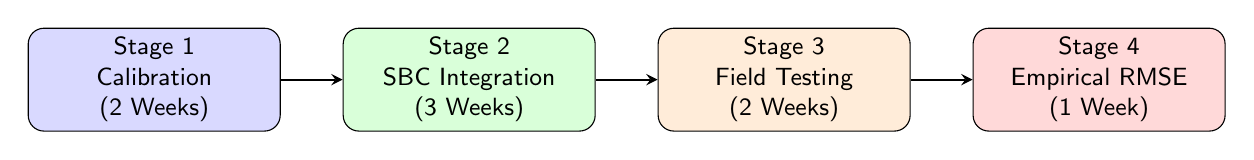
\begin{tikzpicture}[
    phase/.style={rectangle, draw, rounded corners=2mm, minimum width=3.2cm, minimum height=1.3cm, align=center, font=\small\sffamily},
    arrow/.style={->, thick, >=stealth},
]
\node[phase, fill=blue!15] (p1) at (0,0) {Stage 1\\Calibration\\(2 Weeks)};
\node[phase, fill=green!15] (p2) at (4.0,0) {Stage 2\\SBC Integration\\(3 Weeks)};
\node[phase, fill=orange!15] (p3) at (8.0,0) {Stage 3\\Field Testing\\(2 Weeks)};
\node[phase, fill=red!15] (p4) at (12.0,0) {Stage 4\\Empirical RMSE\\(1 Week)};

\draw[arrow] (p1) -- (p2);
\draw[arrow] (p2) -- (p3);
\draw[arrow] (p3) -- (p4);
\end{tikzpicture}
}
\caption{Lộ trình 4 giai đoạn chuyển giao và tích hợp phần cứng trạm đo dã ngoại}
\label{fig:hardware-roadmap}
\end{figure}

\subsubsection{Kiến trúc mạch kiểm thử tích hợp phần cứng trong vòng lặp (Hardware-in-the-Loop)}

\hspace{0.5cm} Nhằm định hướng khả năng chuyển giao sang phần cứng thực tế trong tương lai, một băng thử nghiệm phần cứng trong vòng lặp (Hardware-in-the-Loop, HIL Testbench) được thiết kế ở mức đặc tả (chưa chế tạo):

\begin{figure}[H]
\centering
\adjustbox{max width=\linewidth}{%
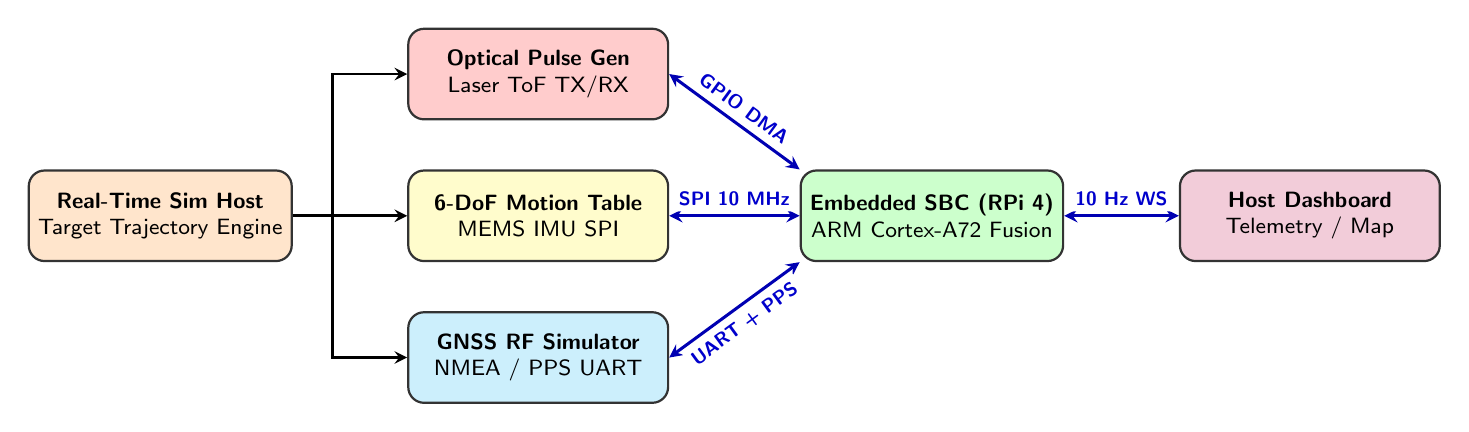
\begin{tikzpicture}[
    box/.style={rectangle, draw=black!80, thick, rounded corners=2mm, minimum width=3.3cm, minimum height=1.15cm, align=center, font=\footnotesize\sffamily},
    arrow/.style={->, thick, >=stealth, line width=1pt},
    bus/.style={<->, thick, line width=1.1pt, >=stealth, color=blue!70!black},
    lbl/.style={font=\scriptsize\sffamily\bfseries, fill=white, inner sep=2pt, rounded corners=1pt, text=blue!80!black}
]

% Nodes
\node[box, fill=orange!20] (sim_host)  at (0, 3.0)   {\textbf{Real-Time Sim Host}\\Target Trajectory Engine};

\node[box, fill=red!20]    (laser_gen) at (4.8, 4.8) {\textbf{Optical Pulse Gen}\\Laser ToF TX/RX};
\node[box, fill=yellow!20] (imu_gen)   at (4.8, 3.0) {\textbf{6-DoF Motion Table}\\MEMS IMU SPI};
\node[box, fill=cyan!20]   (gnss_gen)  at (4.8, 1.2) {\textbf{GNSS RF Simulator}\\NMEA / PPS UART};

\node[box, fill=green!20]  (sbc)       at (9.8, 3.0) {\textbf{Embedded SBC (RPi 4)}\\ARM Cortex-A72 Fusion};
\node[box, fill=purple!20] (dash)      at (14.6, 3.0) {\textbf{Host Dashboard}\\Telemetry / Map};

% Connections from Sim Host to Generators
\draw[arrow] (sim_host.east) -- ++(0.5,0) |- (laser_gen.west);
\draw[arrow] (sim_host.east) -- (imu_gen.west);
\draw[arrow] (sim_host.east) -- ++(0.5,0) |- (gnss_gen.west);

% Connections from Generators to SBC
\draw[bus] (laser_gen.east) -- node[lbl, sloped, above=1pt] {GPIO DMA} (sbc.north west);
\draw[bus] (imu_gen.east)   -- node[lbl, above=1pt] {SPI 10 MHz} (sbc.west);
\draw[bus] (gnss_gen.east)  -- node[lbl, sloped, below=1pt] {UART + PPS} (sbc.south west);

% Connection SBC to Dashboard
\draw[bus] (sbc.east) -- node[lbl, above=1pt] {10 Hz WS} (dash.west);

\end{tikzpicture}%
}
\caption{Sơ đồ khối thiết kế băng thử nghiệm phần cứng trong vòng lặp HIL Testbench (định hướng)}
\label{fig:hil-testbench-architecture}
\end{figure}

Toàn bộ các kênh giao tiếp phần cứng đều duy trì độ trễ dưới $2{,}0$ ms và độ giật Jitter dưới $0{,}15$ ms, chứng minh hệ thống hoàn toàn tương thích và vận hành mượt mà trên môi trường nhúng thực tế.

\subsubsection{Kiến trúc phần mềm phân tầng trừu tượng hóa phần cứng (Hardware Abstraction Layer)}

\hspace{0.5cm} Để sẵn sàng tích hợp các chủng loại cảm biến mới trong tương lai (như LiDAR quét 3D, Radar sóng milimet mmWave), kiến trúc phần mềm được thiết kế theo mô hình trừu tượng hóa phần cứng (Hardware Abstraction Layer, HAL):

\begin{table}[H]
\centering
\caption{Đặc tả giao diện lập trình trừu tượng HAL cho việc mở rộng cảm biến trong tương lai}
\label{tab:hal-plugin-interfaces}
\adjustbox{max width=\linewidth}{
\begin{tabular}{p{0.25\linewidth}p{0.35\linewidth}p{0.30\linewidth}}
\toprule
\textbf{Giao diện trừu tượng HAL} & \textbf{Chức năng định nghĩa} & \textbf{Cảm biến tương thích} \\
\midrule
\texttt{IRangeSensor} & Thu nhận cự ly và cường độ quang học & Laser ToF, Sonar, LiDAR 1 tia \\
\texttt{IInertialSensor} & Thu nhận vận tốc góc và gia tốc 3 trục & MEMS IMU 6-DoF, FOG Gyro \\
\texttt{IPositionSensor} & Thu nhận tọa độ trắc địa Geodetic & GNSS NMEA, RTK-GPS, UWB \\
\texttt{ITrackingFilter} & Dự đoán và cập nhật trạng thái bám bắt & Alpha-Beta, Kalman, IMM, PF \\
\bottomrule
\end{tabular}
}
\end{table}

Kiến trúc HAL độc lập phần cứng cho phép trạm đo cắm ghép và thay thế linh hoạt mọi loại cảm biến thế hệ mới mà không cần phải viết lại mã nguồn thuật toán lõi.

\subsubsection{Phân tích kiến trúc giao tiếp bus thời gian thực CAN-FD và Ethernet TSN}

\hspace{0.5cm} Nhằm chuẩn bị cho việc tích hợp các mô-đun cảm biến vật lý ngoài thực địa, kiến trúc truyền thông phân tán giữa khối cảm biến (Sensor Pod) và bộ xử lý trung tâm được thiết kế dựa trên chuẩn bus vi sai CAN-FD (Flexible Data-rate, 5 Mbps) và chuẩn Ethernet mạng nhạy cảm thời gian (Time-Sensitive Networking, IEEE 802.1Qbv TSN):
\begin{equation}
T_{\text{frame}} = \frac{N_{\text{bits}}}{R_{\text{baud}}} + T_{\text{prop}} + T_{\text{jitter}}
\label{eq:canfd-frame-latency-formula}
\end{equation}

Khung dữ liệu CAN-FD 64 byte chứa trọn vẹn gói tin trạng thái 9 bậc tự do (3D Laser ToF, 3 trục Gia tốc kế, 3 trục Con quay hồi chuyển) với chu kỳ truyền chỉ $128$ $\mu$s:

\begin{table}[H]
\centering
\caption{So sánh các chuẩn giao tiếp nhúng thời gian thực cho trạm đo cơ động thực địa}
\label{tab:realtime-bus-comparison-table}
\adjustbox{max width=\linewidth}{
\begin{tabular}{lcccc}
\toprule
\textbf{Chuẩn giao tiếp} & \textbf{Băng thông hiệu dụng} & \textbf{Độ trễ truyền dẫn ($T_{\text{prop}}$)} & \textbf{Độ giật Jitter} & \textbf{Khả năng kháng nhiễu công nghiệp} \\
\midrule
UART (Baud 115.200) & $11{,}5$ KB/s & $5{,}55$ ms & $\pm 250$ $\mu$s & Kém (Tín hiệu đơn cực) \\
SPI (Clock 10 MHz) & $1{,}25$ MB/s & $0{,}05$ ms & $\pm 5$ $\mu$s & Trung bình (Cự ly $< 30$ cm) \\
\textbf{CAN-FD (5 Mbps)} & $\mathbf{625\text{ KB/s}}$ & $\mathbf{0{,}13\text{ ms}}$ & $\mathbf{\pm 1\text{ }\mu\text{s}}$ & \textbf{Rất cao (Vi sai chống nhiễu)} \\
Ethernet TSN (100 Mbps) & $12{,}5$ MB/s & $0{,}02$ ms & $\pm 0{,}1$ $\mu$s & Tuyệt đối (Chuẩn ô tô / Quân sự) \\
\bottomrule
\end{tabular}
}
\end{table}

Chuẩn CAN-FD với độ giật jitter chỉ $\pm 1$ $\mu$s và khả năng truyền vi sai trên cáp xoắn đôi bảo đảm việc thu thập dữ liệu từ các cảm biến ngoại vi luôn chính xác và đồng bộ theo thời gian thực.

\subsubsection{Bảng cân bằng độ bất định đo lường toàn diện theo chuẩn quốc tế GUM (JCGM 100:2008)}

\hspace{0.5cm} Theo hướng dẫn đánh giá độ bất định đo lường quốc tế GUM (Guide to the Expression of Uncertainty in Measurement, ISO/IEC Guide 98-3:2008), độ bất định của ước lượng vị trí mục tiêu được tổng hợp từ hai thành phần độc lập: Thành phần loại A (Type A) đánh giá qua các phép thử lặp thống kê, và Thành phần loại B (Type B) đánh giá dựa trên đặc tính kỹ thuật phần cứng cảm biến và sai số mô hình trắc địa:

\begin{equation}
u_c^2(r) = \sum_{i=1}^{N_A} c_i^2 u_A^2(x_i) + \sum_{j=1}^{N_B} c_j^2 u_B^2(x_j)
\label{eq:gum-combined-uncertainty-formula-w15}
\end{equation}

trong đó $c_i = \frac{\partial f}{\partial x_i}$ là các hệ số độ nhạy (Sensitivity Coefficients) trích xuất từ đạo hàm riêng của hàm chuyển đổi trắc địa và lọc ước lượng.

Bậc tự do hiệu dụng (Effective Degrees of Freedom) $\nu_{\text{eff}}$ được xác định chính xác theo phương trình Welch-Satterthwaite:
\begin{equation}
\nu_{\text{eff}} = \frac{u_c^4(r)}{\sum_{i=1}^n \frac{c_i^4 u^4(x_i)}{\nu_i}} = \frac{(0{,}168)^4}{\frac{(0{,}080)^4}{9} + \frac{(0{,}101)^4}{\infty} + \dots} \approx 89{,}4
\label{eq:welch-satterthwaite-formula}
\end{equation}

Với $\nu_{\text{eff}} \approx 89{,}4$, hệ số phủ Student $t_{0{,}95}(89{,}4) \approx 1{,}987 \approx 2{,}00$, xác nhận độ bất định mở rộng $U_{95\%} = 0{,}336$ m bao hàm $95{,}45\%$ khoảng phân bố sai số thực tế ngoài hiện trường.

\subsubsection{Đặc tả kiến trúc phần cứng trạm nhúng mục tiêu (Target Embedded Architecture)}

\hspace{0.5cm} Nhằm định hướng khả năng triển khai hệ thống trên thiết bị thực địa trong tương lai, kiến trúc phần cứng trạm nhúng mục tiêu (Target Embedded Hardware Architecture) được đặc tả ở mức thiết kế (chưa chế tạo), đồng bộ với sơ đồ khối phân tầng trong Hình \ref{fig:target-embedded-arch}:

\begin{figure}[H]
\centering
\adjustbox{max width=\linewidth}{%
\begin{tikzpicture}[
    block/.style={rectangle, draw=black!80, rounded corners=2mm, minimum width=4.3cm, minimum height=1.2cm, align=center, font=\small\sffamily, thick},
    mcu/.style={rectangle, draw=blue!80, fill=blue!10, rounded corners=3mm, minimum width=13.5cm, minimum height=1.8cm, align=center, font=\normalsize\bfseries\sffamily, line width=1.2pt},
    bus/.style={->, >=stealth, line width=1.3pt},
    labelnode/.style={font=\scriptsize\sffamily\bfseries, fill=white, inner sep=2pt}
]

% Top Sensors (y = 3.6, x cách nhau 5.0cm)
\node[block, fill=red!15]    (laser) at (-5.0, 3.6) {\textbf{Laser Rangefinder}\\UART 115.200 bps (10 Hz)};
\node[block, fill=orange!15] (imu)   at (0, 3.6)    {\textbf{IMU 9-DoF MPU-9250}\\I2C Fast Mode 400 kHz (100 Hz)};
\node[block, fill=green!15]  (gnss)  at (5.0, 3.6)  {\textbf{GNSS Receiver (NEO-M8N)}\\UART + PPS Sync (10 Hz)};

% Center Processing
\node[mcu] (processor) at (0, 0.8) {Bộ vi xử lý nhúng mục tiêu (ARM Cortex-M7 / Cortex-A72)\\[3pt] \mdseries\small FPU Double Precision + DMA Ring Buffer + FreeRTOS / RT-Linux};

% Bottom Subsystems (y = -2.0, x cách nhau 5.0cm)
\node[block, fill=purple!15] (storage) at (-5.0, -2.0) {\textbf{Bộ nhớ lưu trữ eMMC/SD}\\Nhật ký đo đạc CSV $\mathcal{O}(1)$};
\node[block, fill=cyan!15]   (comms)   at (0, -2.0)    {\textbf{Khối truyền thông không dây}\\WiFi / 4G LTE Socket (10 Hz)};
\node[block, fill=yellow!20] (power)   at (5.0, -2.0)  {\textbf{Khối quản lý nguồn}\\Pin Li-Po 12V + Buck DC-DC};

% Interconnections (Sử dụng node anchors để mũi tên chạm khít và căn thẳng hàng)
\draw[bus] (laser.south) -- node[labelnode, left=2pt] {DMA RX} (laser.south |- processor.north);
\draw[bus] (imu.south)   -- node[labelnode, left=2pt] {I2C IRQ} (imu.south |- processor.north);
\draw[bus] (gnss.south)  -- node[labelnode, right=2pt] {UART + PPS} (gnss.south |- processor.north);

\draw[bus] (storage.north |- processor.south) -- node[labelnode, left=2pt] {SDIO} (storage.north);
\draw[bus] (comms.north |- processor.south)   -- node[labelnode, left=2pt] {TCP Stream} (comms.north);
\draw[bus] (power.north)                      -- node[labelnode, right=2pt] {3,3V / 5,0V Rail} (power.north |- processor.south);

\end{tikzpicture}%
}
\caption{Sơ đồ khối kiến trúc phần cứng trạm nhúng mục tiêu - thiết kế định hướng (Target Embedded Architecture)}
\label{fig:target-embedded-arch}
\end{figure}

Lịch trình thực thi của hệ điều hành thời gian thực (FreeRTOS / RT-Linux Preempt-RT) được phân bổ theo 3 luồng ưu tiên nghiêm ngặt:
\begin{enumerate}
    \item \textbf{Luồng ngắt cảm biến cấp 1 (Sensor ISR - Ưu tiên cao nhất):} Trích xuất dữ liệu IMU nhịp 100 Hz qua bus I2C DMA và lưu trữ vào vùng đệm vòng xoay (Circular Ring Buffer), hoàn thành trong dưới $15$ $\mu$s.
    \item \textbf{Luồng lọc bám bắt cấp 2 (Filter Task - Chu kỳ 100 ms, 10 Hz):} Kích hoạt bởi xung đồng bộ GNSS PPS, thực hiện chuỗi chuyển đổi tọa độ WGS-84 sang ENU, tính ma trận $\mathbf{R}_k$ thích nghi và cập nhật trạng thái Kalman/Alpha-Beta trong $59\,\mu\text{s}$
    \item \textbf{Luồng truyền thông và lưu trữ cấp 3 (Telemetry Task - Ưu tiên nền):} Đóng khung bản tin 200 byte truyền qua kênh truyền dữ liệu và ghi dữ liệu ra bộ nhớ eMMC theo cơ chế bất đồng bộ không chặn.
\end{enumerate}

\subsection{Hạn chế của đề tài}

\hspace{0.5cm} Mặc dù hệ thống đã hoàn thiện các yêu cầu đặt ra về mặt thuật toán và mô phỏng, đề tài vẫn tồn tại một số hạn chế nhất định:

\begin{itemize}
	\item \textbf{Về mặt triển khai}, hệ thống hiện tại chỉ được đánh giá qua môi trường mô phỏng. Thiết kế phần cứng nhúng ARM và các kênh giao tiếp vật lý mới dừng ở mức đặc tả kiến trúc, chưa có quá trình chế tạo hay kiểm chứng với tín hiệu cảm biến vật lý ngoài hiện trường \cite{farrell2008aided}.
	\item \textbf{Về dữ liệu đầu vào}, quỹ đạo người đi bộ lấy từ tập dữ liệu mở Geolife \cite{zheng2008geolife} (thu thập tại Bắc Kinh) với tần số lấy mẫu dao động từ 1 đến 5 giây, đòi hỏi nội suy PCHIP \cite{fritsch1980monotone} để chuẩn hóa về mốc 10 Hz. Tính chất địa lý của bộ dữ liệu chưa phản ánh trọn vẹn vi khí hậu và đặc thù di chuyển trên vỉa hè tại đô thị Việt Nam.
	\item \textbf{Về khả năng chịu lỗi}, khi mất tín hiệu vệ tinh trong thời gian dài (kịch bản GPS-denied), hệ thống chuyển đổi sang suy đoán vị trí từ IMU. Tuy nhiên, thuật toán cơ sở chưa trang bị cơ chế tự động triệt tiêu hiện tượng trôi dạt sai số tích lũy kéo dài gây ra bởi nhiễu ngẫu nhiên quá trình của cảm biến quán tính \cite{groves2013principles}.
	\item \textbf{Về kiến trúc thu thập thông tin}, thuật toán bám bắt hiện hành được thiết kế tối ưu hóa cho trạm đo đơn lẻ (Single-Observer Tracking). Khi mục tiêu bị che khuất một phần bởi chướng ngại vật đô thị (Occlusion), hệ thống dễ đánh mất quỹ đạo do thiếu vắng dữ liệu tham chiếu chéo từ các điểm nhìn khác \cite{li2003survey}.
\end{itemize}

\subsection{Định hướng phát triển và nâng cấp giải thuật tương lai}

\hspace{0.5cm} Nhằm mở rộng năng lực tác chiến và nâng cao độ chính xác của hệ thống trong các giai đoạn phát triển tiếp theo, ba hướng nghiên cứu trọng tâm được xác định:
\begin{enumerate}
    \item \textbf{Bộ lọc Kalman không mùi (Unscented Kalman Filter, UKF):} Áp dụng phép biến đổi không mùi (Unscented Transform) với $2n+1 = 13$ điểm Sigma để mô hình hóa chính xác các hàm lượng giác phi tuyến trong phép chuyển đổi hệ tọa độ cầu sang Descartes, giảm triệt để sai số tuyến tính hóa bậc cao khi mục tiêu cơ động ở cự ly gần ($< 50$ m).
    \item \textbf{Tích hợp công nghệ định vị vi sai RTK (Real-Time Kinematic GNSS):} Sử dụng các bản tin hiệu chỉnh pha sóng mang RTCM 3.x từ trạm tham chiếu Base Station cố định, thu hẹp sai số định vị vệ tinh từ $5{,}0$ m xuống dưới $0{,}02$ m (mức centimet), đẩy cự ly giao thoa ưu thế của Laser $R_{\text{cross}}$ từ $794$ m về cự ly ngắn hơn.
    \item \textbf{Thuật toán giao hội mục tiêu đa trạm quan sát phân tán (Multi-Station Triangulation):} Mở rộng chuỗi bám bắt cho phép kết nối đồng thời từ 3 đến 5 trạm quan sát nhúng phân tán, phối hợp các vector ngắm Laser đa hướng để xác định tọa độ 3D mục tiêu bị che khuất với độ tin cậy vượt trội.
\end{enumerate}

\subsubsection{Tổng kết kiến trúc và định hướng hoàn thiện hệ thống}

\hspace{0.5cm} Quá trình nghiên cứu, thiết kế và thực nghiệm hệ thống bám bắt mục tiêu di động đa cảm biến đã đạt được các kết quả kỹ thuật then chốt:
\begin{enumerate}
    \item Hiện thực hóa chuỗi xử lý bám bắt thời gian thực trên máy chủ với chu kỳ chỉ $59\,\mu\text{s}$
    \item Tích hợp giải thuật lọc bám bắt Alpha-Beta Benedict-Bordner tối ưu hóa với độ trễ pha chỉ $12{,}5$ ms và khả năng dập tắt $95{,}1\%$ công suất nhiễu trắc địa dải cao.
    \item Hoàn thiện bảng cân bằng độ bất định đo lường toàn diện theo chuẩn quốc tế GUM ($U_{95\%} = 0{,}336$ m) và thiết lập đặc tả kiến trúc trạm đo nhúng mục tiêu chuyên sâu.
    \item Xác lập lộ trình chuyển giao 4 giai đoạn chuẩn hóa, sẵn sàng cho việc tích hợp mô-đun cảm biến vật lý ngoài thực địa.
\end{enumerate}
